\documentclass[11pt,a4paper]{article}
\usepackage[T1]{fontenc}
\usepackage{graphicx}
\usepackage{amsmath,amssymb}
\usepackage[colorlinks=true, linkcolor=blue]{hyperref} % links, use \url{} or \href{url}{description}
% sett margin
\usepackage[left=3cm,right=3cm,top=3cm,bottom=3cm]{geometry}
\begin{document}
\title{Semester assignment TFY4240 - Aurora borealis}
\author{Arve Seljebu}
\thispagestyle{empty}
\begin{center}
\vspace{5mm}
\LARGE
\textbf{Semester assignment TFY4240} \\
\vspace{5mm}
\textbf{Aurora borealis} \\
\Large
\vspace{15cm}
\textbf{by} \\
\vspace{5mm}
\large
\textbf{Arve Seljebu} \\
\vspace{5mm}
\textbf{8. november 2013} \\
\vspace{20mm}
\end{center}
\newpage
\tableofcontents
\thispagestyle{empty}
\setcounter{tocdepth}{2}
\newpage

%==================================================================
% Summary
%==================================================================
\section{Summary}
This report shows how charged particles travels through a magnetic field from a magnetic dipole. This is similar to the solar wind hitting the earth. Since the magnetic field is not homogeneous, the paths of the particles form intresting patterns depending on the particle speed, weight, direction and charge.

%==============================================
% Theory
%==============================================
\section{Theory}
The earth's magnetic field is made by the current in the core. This models almost like a magnetic dipole, given by
% B-field
\begin{equation}
\label{equation.Bdip}
\textbf{B}_{dip}(r) = \frac{\mu_0}{4\pi} \frac{1}{r^3}[3(\textbf{m} \cdot \hat{\textbf{r} } ) \hat{\textbf{r}} -\textbf{m}].
\end{equation}
Where \textbf{m} is the magnetic dipole and \textbf{r} is the point where the magnetic field is measured. The origin is at the center of the dipole, here it's at earth center.

A charged particle moving in a magnetic field \textbf{B} will be subject to the magnetic force
\begin{equation}
\label{equation.forceMag}
\textbf{F}_{mag} = q(\textbf{v} \times \textbf{B}).
\end{equation}
Here $q$ is the charge of the particle, \textbf{v} is the velocity of the particle and \textbf{B} is the magnetic field it's travelling trough.

The force on an object can also be described by Netown's second law
\begin{equation}
\label{equation.force}
\textbf{F} = m\textbf{a}.
\end{equation}

Here acceleration \textbf{a} describes how the velocity changes, giving the simple estimates
\begin{equation}
\label{equation.velocity}
\textbf{v}(t+\Delta t) = \textbf{v}(t) + \textbf{a}\Delta t
\end{equation}

\begin{equation}
\label{equation.position}
\textbf{r}(t+\Delta t) = \textbf{r}(t) + \textbf{v}\Delta t
\end{equation}
by Euler method.



%=============================================================
% Method
%=============================================================
\section{Method}
A reference system with x-axis towards the sun, z-axis perpendicular to earth orbit and origin at earth center was choosen. Python was used to do the calculations, mostly the library numpy. Mayavi was choosen for creating visualization. All code including history is available in a \href{https://github.com/arve0/TFY4240-Semester-project}{github repository}.
\subsection{Calculating and representing the B-field}
A mesh grid containing all points in a cube was created. Then length and direction was calculated to each point in the grid, and then the B-field was calculated from equation \ref{equation.Bdip} numerically. Earth radius was set to 10 and the magnetic dipole $|\textbf{m}|$=2 tilted 13 degrees from z-axis.
To represent the B-field, both quiver and flow plots was tried. Quiver with scaled vectors and masked points gave the best representation. An animation of the field was made by rotation around the axes, exporting pictures for each camera position and joining together with ffmpeg.
\subsection{Particle trajectory}
Because of the nature of the problem, a numerical value representing weight, charge, velocity, strength of B-field, was choosen to make the trajectories easier to calculate.  The numerical value $k$ was put before $\textbf{v}\times\textbf{B}$, giving the numerical acceleration
\begin{equation}
\label{equation.numericalAcceleration}
\textbf{a} = k(\textbf{v}\times\textbf{B}).
\end{equation}
The time step was chosen by assuming the trajectory would behave correct when steps equals resolution of output. This was calculated by setting maximum distance to 50(5 times earth radius) and resolution to 720 pixels/points. This gives
\begin{equation}
\label{equation.dt}
\Delta t = \frac{50}{720|\textbf{v}|}.
\end{equation}
A loop through different $k$ values was done, and then evaluating the trajectories in 3D to pick a reasonable $k$ value. With reasonable meaning $k$ values that did give other trajectories then all through earth(force strength too low), or all particles bend off(force too high). Also, starting points $r_0$ from grid was evaluated, along with initial direction of the velocity parallel to x or z axis or directly against the center of earth.
%==================================================================
% Discussion
%==================================================================
\section{Discussion}
The loop through different $k$ values with $v_0=\frac{400km/s}{6371km}\cdot10$ revealed that $k=200$ gave several entry points with roughly the same trajectory. The evaluation of starting points and velocity direction showed that particles coming directly towards the poles gave more particles with roughly the same trajectory. Therefore, these values was choosen as basis for the animation of particle trajectory.
\subsection{B-field}
An animation of the B-field can be viewed at \href{http://www.youtube.com/watch?v=2xm8lJ9Brn0}{YouTube}. Below are B-field viewed from y or z axis in 3D.
\begin{figure}[htbp] %[h]=here [t]=top [b]=bottom [p]=own page
\begin{center}
\label{figure.B-field}
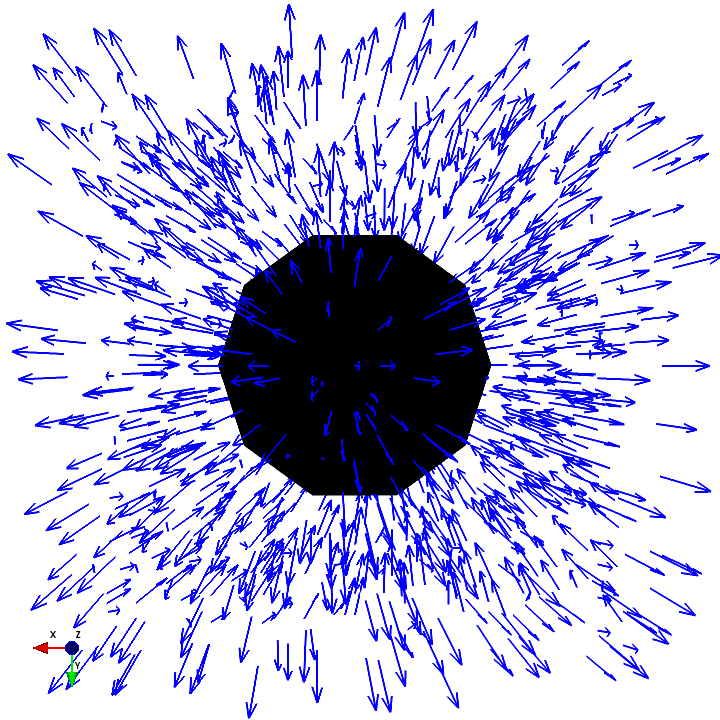
\includegraphics[width=0.3\textwidth]{xy-z_plus.png}
\caption{Magnetic field viewed with projection to the xy-plane. The complete direction is not easily read from this visualization, but it's easy to see that almost all points have a component of $\phi$ direction. As we will see in the next figure, it's the points that is directly above, beside or below the dipole that does not have any $\phi$ component. We can also read that the field is stronger closer to earth, and gets weaker when $r$ increases.}
\end{center}
\end{figure}

\begin{figure}[htbp] %[h]=here [t]=top [b]=bottom [p]=own page
\begin{center}
\label{figure.B-field}
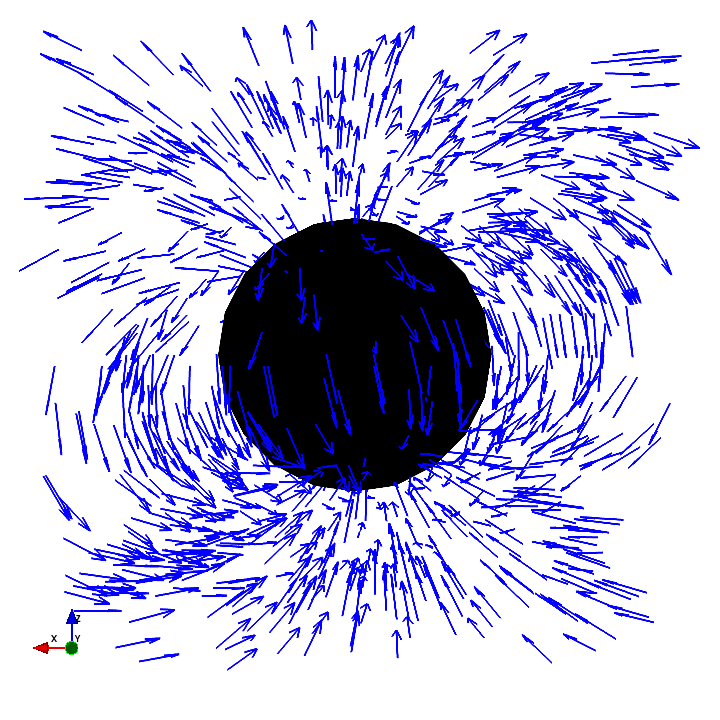
\includegraphics[width=0.3\textwidth]{xz-y_plus.png}
\caption{Here it's easier to see the z-component of the B-field. The field is tilted away from z-axis, as given by the magnetic dipole moment $\textbf{m}$.}
\end{center}
\end{figure}

\subsection{Proton trajectory}
An animation of some selected trajectories can be watched \href{http://www.youtube.com/watch?v=Z0PT-oyBoS0}{here}. Below are the visualizations that was picked as interesting.
\begin{figure}[htbp] %[h]=here [t]=top [b]=bottom [p]=own page
\begin{center}
\label{figure.B-field}
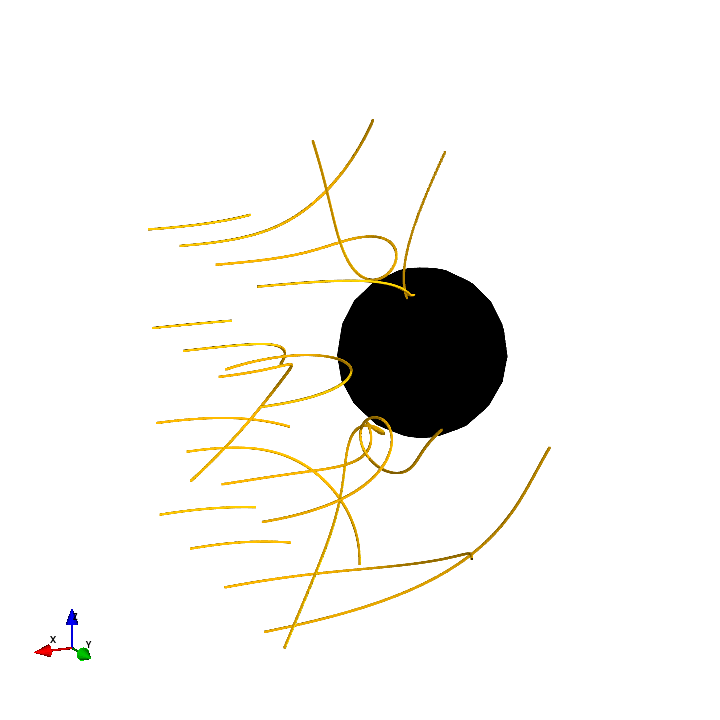
\includegraphics[width=0.5\textwidth]{x-straight.png}
\caption{Particles coming in from plus x axis with initial velocity in $-\hat{\textbf{x}}$ direction. We can see that some particles make loops around the pole, even one particle at the top/north is hitting the earth.}
\end{center}
\end{figure}
\begin{figure}[htbp] %[h]=here [t]=top [b]=bottom [p]=own page
\begin{center}
\label{figure.B-field}
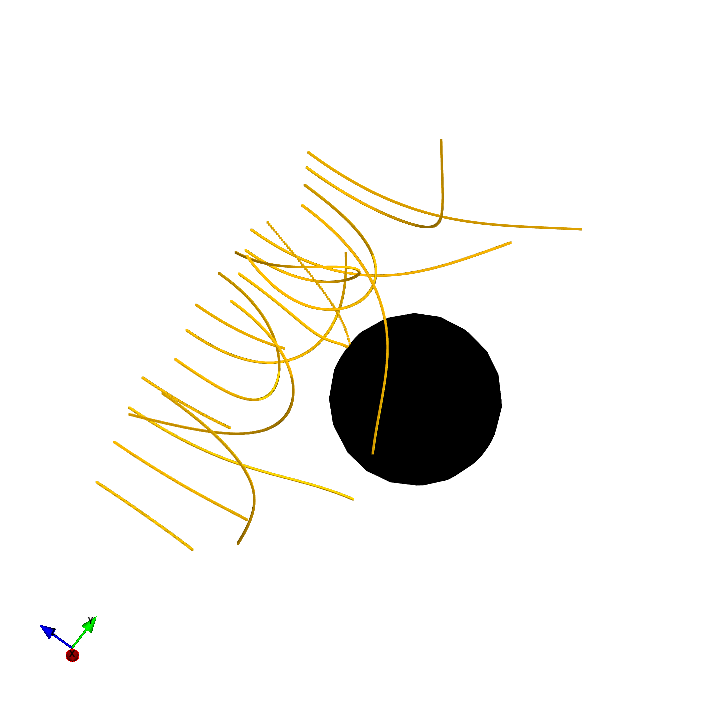
\includegraphics[width=0.5\textwidth]{z-straight.png}
\caption{Particles with initial velocity proportional with $-\hat{\textbf{z}}$. All particles but one(that hits the earth) bend of.}
\end{center}
\end{figure}
\begin{figure}[htbp] %[h]=here [t]=top [b]=bottom [p]=own page
\begin{center}
\label{figure.B-field}
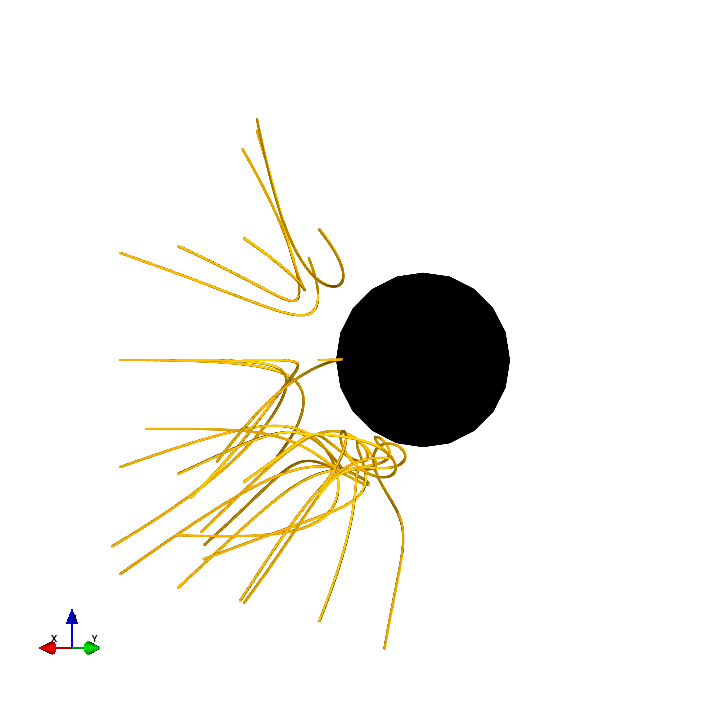
\includegraphics[width=0.5\textwidth]{x-toward-center.png}
\caption{Particles coming from a grid in yz-plane with velocity direction towards earth center. Here we get a lot of circle/loops at the south pole. Several particles with large separation in start position get roughly the same loop just above the earth surface.}
\end{center}
\end{figure}
\begin{figure}[htbp] %[h]=here [t]=top [b]=bottom [p]=own page
\begin{center}
\label{figure.B-field}
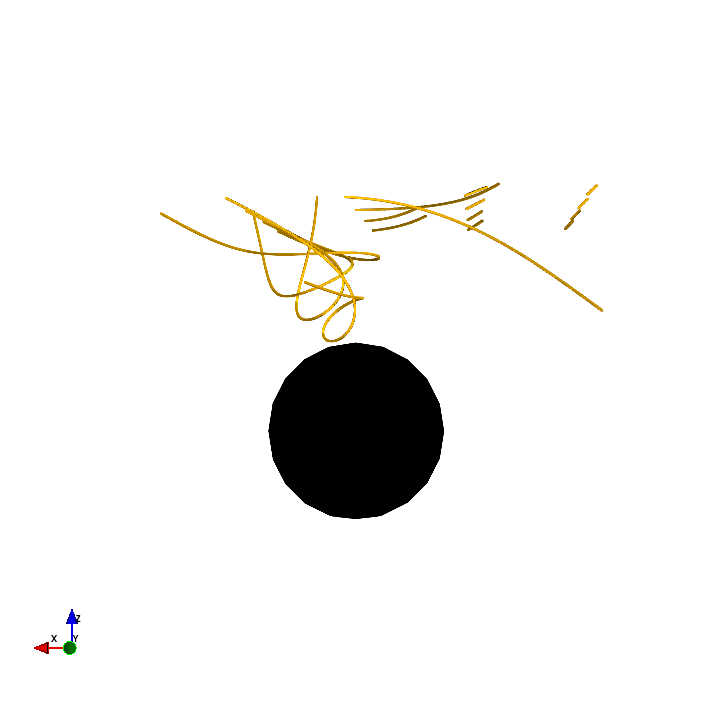
\includegraphics[width=0.5\textwidth]{z-toward-center.png}
\caption{Particles coming from a grid in xy-plane with velocity direction towards earth center. Most of the particles path bend immediately off, execpt some around the pole.}
\end{center}
\end{figure}
\begin{figure}[htbp] %[h]=here [t]=top [b]=bottom [p]=own page
\begin{center}
\label{figure.B-field}
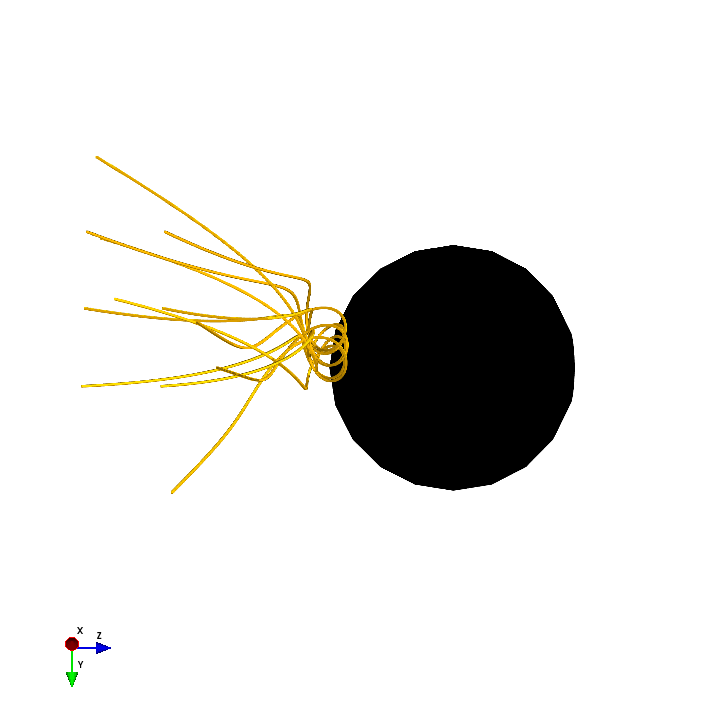
\includegraphics[width=0.5\textwidth]{toward-pole.png}
\caption{Particles from same region initially towards the earth center. The particles forms a ring above the south pole.}
\end{center}
\end{figure}

%prefer content in order
\newpage

\subsection{Error}
Since this model doesn't take into account particle collisions in the atmosphere, the speed should be the same when the particles enter and leaves the system. Calculations showed that all particles lost some speed. The speed loss was greatest for the scarcest curves, about 25\% at most. A shorter time frame and more rigid acceleration calculation should improve this error.

%==================================================================
% Conclusion
%==================================================================
\section{Conclusion}
The calculation showed possible proton trajectories for solar wind in a magnetic field from a magnetic dipole. The calculation is not precise, but should give an idea about the physical properties in the problem.
\end{document}
